\documentclass[%
  border=1mm
%  border={0pt 0pt 0pt 0pt} % left bottom right top
]{standalone}% http://ctan.org/pkg/standalone

\usepackage{tikz}
\usepackage{wasysym} % for \lightning

% packages we need for platform detection
\usepackage{pdftexcmds}
\usepackage{catchfile}
\usepackage{ifluatex}
\usepackage{ifplatform}
\usepackage{fontspec}
\iflinux
\setmainfont{Roboto}
\setsansfont{Roboto}
\else
\setmainfont{PT Sans}
\setsansfont{PT Sans}
\fi

\newcommand*{\defaulttextstyle}{\sffamily\Large\bfseries\color{black!85}}
\newcommand*{\bigtextstyle}{\sffamily\huge\bfseries\color{black!85}}


%\usepackage[defaultsans]{droidsans}
%\renewcommand*\familydefault{\sfdefault} %% Only if the base font of the document is to be typewriter style
%\usepackage[T1]{fontenc}

\newcommand\centerdrillmark{} % just for safety
\def\centerdrillmark{
  \draw [dashed] (0,2.5mm) -- (0,-2.5mm);
	\draw [dashed]  (2.5mm,0) -- (-2.5mm,0);
}

\usetikzlibrary{decorations.text}
\definecolor{mygray}{RGB}{208,208,208}
\newcommand{\arcarrow}[3]{%
   % inner radius, middle radius, outer radius, start angle,
   % end angle, tip protusion angle, options, text
   \pgfmathsetmacro{\rin}{0.8}
   \pgfmathsetmacro{\rmid}{1.6}
	 \pgfmathsetmacro{\rout}{2.0}
   \pgfmathsetmacro{\astart}{#1}
   \pgfmathsetmacro{\aend}{#2}
   \fill[mygray, very thick] (\astart:\rin)
                         arc (\astart:\aend:\rin)
      -- (\aend:\rmid)
      -- (\aend:\rout)   arc (\aend:\astart:\rout)
      -- (\astart:\rmid) -- cycle;

		\node[font=\large] at (\angle:16mm) {\defaulttextstyle{#3}};
   %\path[
   %   decoration = {
   %      text along path,
   %      text = {|\defaulttextstyle|#3},
   %      text align = {align = center},
   %      raise = -1.0ex
   %   },
   %   decorate
   %](\astart:\rmid) arc (\astart:\aend:\rmid);
}

\begin{document}

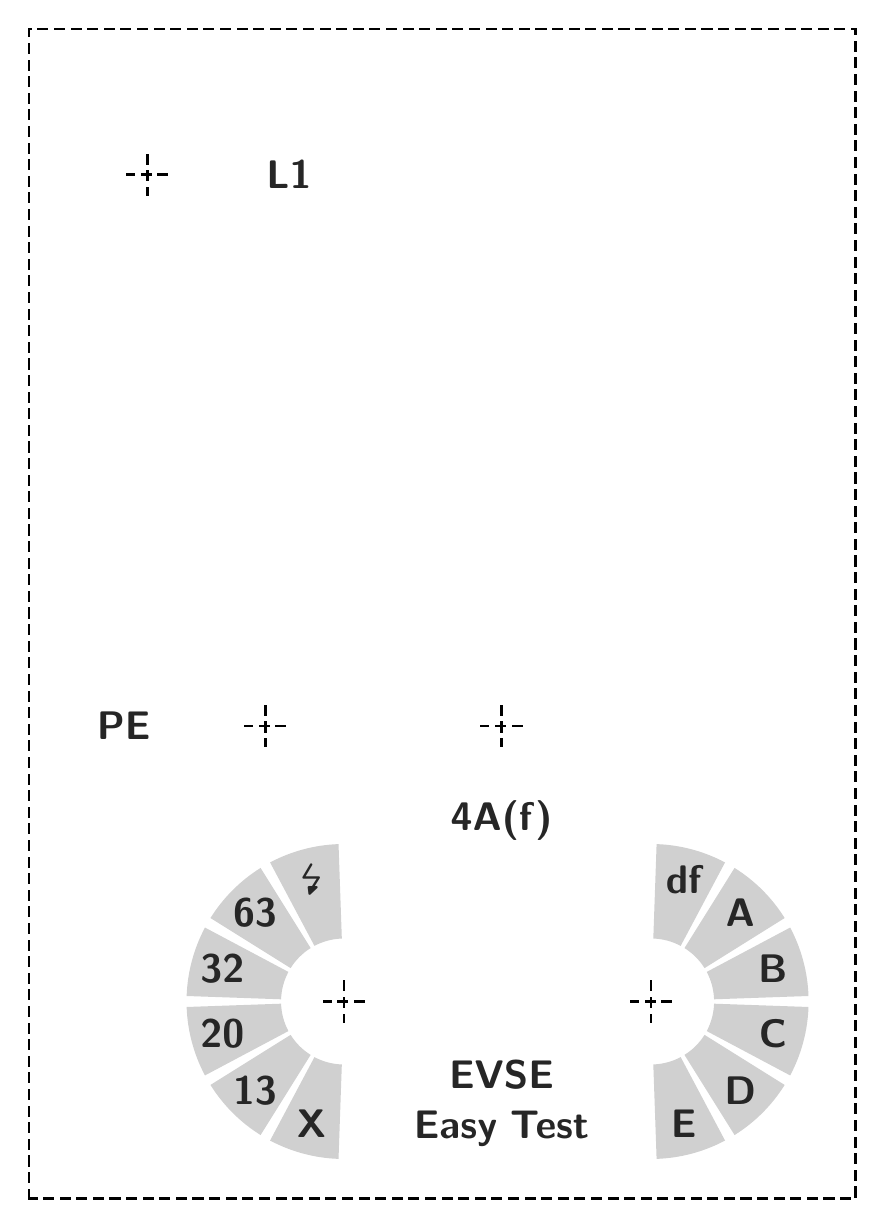
\begin{tikzpicture}[line cap=rect,line width=1pt]

% Outer Frame: Quarter of A4 paper: 10.5cm x 14.85cm
\draw [dashed] (0,0) --
	(0mm,148.5mm) --
	(105mm,148.5mm) --
	(105.0mm,0mm) --
	cycle;

% Product name
\begin{scope}[shift={(60mm,12mm)}]
	\node[align=center, font=\Large, text width=25mm] at (0:0mm)
	{\defaulttextstyle{{EVSE Easy Test}}};
\end{scope}

% PE switch
\begin{scope}[shift={(30mm,60mm)}]
	\centerdrillmark;
	\node[font=\large] at (180:18mm) {\defaulttextstyle{PE}};
\end{scope}

% Fuse
\begin{scope}[shift={(60mm,60mm)}]
	\centerdrillmark;
	\node[font=\large] at (270:12mm) {\defaulttextstyle{4A(f)}};
\end{scope}

% L1 LED
\begin{scope}[shift={(15mm,130mm)}]
	\centerdrillmark
	\node[font=\large] at (0:18mm) {\defaulttextstyle{L1}};
\end{scope}


% State dial
\begin{scope}[shift={(79mm,25mm)}]
	%\draw (0,0) circle [radius=10mm];
	\centerdrillmark
	\foreach \angle/\label [count=\xi] in 
	{
		75/{df},45/A,15/B,-15/C,-45/D,-75/E
	}
	{
		%\draw[line width=2pt] (\angle:10mm) -- (\angle:15mm);
		%\node[font=\large] at (\angle:18mm) {\textsf{\label}};
		\arcarrow{\angle+13}{\angle-13}{\label}
	}
\end{scope}

% Max current dial
\begin{scope}[shift={(40mm,25mm)}]
	%\draw (0,0) circle [radius=10mm];
	\centerdrillmark
	\foreach \angle/\label [count=\xi] in
	{
		180-75/{\lightning},180-45/63,180-15/32,180+15/20,180+45/13,180+75/{X}
	}
	{
		%\draw[line width=2pt] (\angle:10mm) -- (\angle:15mm);
		%\node[font=\large] at (\angle:18mm) {\textsf{\label}};
		\arcarrow{\angle+13}{\angle-13}{\label}
	}
\end{scope}



\end{tikzpicture}

\end{document}
